% Options for packages loaded elsewhere
\PassOptionsToPackage{unicode}{hyperref}
\PassOptionsToPackage{hyphens}{url}
\PassOptionsToPackage{dvipsnames,svgnames,x11names}{xcolor}
\documentclass[
  12pt,
  a4paper,
]{article}
\usepackage{xcolor}
\usepackage[top=2.5cm,bottom=2.5cm,left=3cm,right=2cm]{geometry}
\usepackage{amsmath,amssymb}
\setcounter{secnumdepth}{5}
\usepackage{iftex}
\ifPDFTeX
  \usepackage[T1]{fontenc}
  \usepackage[utf8]{inputenc}
  \usepackage{textcomp} % provide euro and other symbols
\else % if luatex or xetex
  \usepackage{unicode-math} % this also loads fontspec
  \defaultfontfeatures{Scale=MatchLowercase}
  \defaultfontfeatures[\rmfamily]{Ligatures=TeX,Scale=1}
\fi
\usepackage{lmodern}
\ifPDFTeX\else
  % xetex/luatex font selection
    \setmainfont[]{Times New Roman}
    \setmonofont[Scale=0.85]{Liberation Mono}
\fi
% Use upquote if available, for straight quotes in verbatim environments
\IfFileExists{upquote.sty}{\usepackage{upquote}}{}
\IfFileExists{microtype.sty}{% use microtype if available
  \usepackage[]{microtype}
  \UseMicrotypeSet[protrusion]{basicmath} % disable protrusion for tt fonts
}{}
\makeatletter
\@ifundefined{KOMAClassName}{% if non-KOMA class
  \IfFileExists{parskip.sty}{%
    \usepackage{parskip}
  }{% else
    \setlength{\parindent}{0pt}
    \setlength{\parskip}{6pt plus 2pt minus 1pt}}
}{% if KOMA class
  \KOMAoptions{parskip=half}}
\makeatother
\usepackage{color}
\usepackage{fancyvrb}
\newcommand{\VerbBar}{|}
\newcommand{\VERB}{\Verb[commandchars=\\\{\}]}
\DefineVerbatimEnvironment{Highlighting}{Verbatim}{commandchars=\\\{\}}
% Add ',fontsize=\small' for more characters per line
\newenvironment{Shaded}{}{}
\newcommand{\AlertTok}[1]{\textcolor[rgb]{1.00,0.00,0.00}{\textbf{#1}}}
\newcommand{\AnnotationTok}[1]{\textcolor[rgb]{0.38,0.63,0.69}{\textbf{\textit{#1}}}}
\newcommand{\AttributeTok}[1]{\textcolor[rgb]{0.49,0.56,0.16}{#1}}
\newcommand{\BaseNTok}[1]{\textcolor[rgb]{0.25,0.63,0.44}{#1}}
\newcommand{\BuiltInTok}[1]{\textcolor[rgb]{0.00,0.50,0.00}{#1}}
\newcommand{\CharTok}[1]{\textcolor[rgb]{0.25,0.44,0.63}{#1}}
\newcommand{\CommentTok}[1]{\textcolor[rgb]{0.38,0.63,0.69}{\textit{#1}}}
\newcommand{\CommentVarTok}[1]{\textcolor[rgb]{0.38,0.63,0.69}{\textbf{\textit{#1}}}}
\newcommand{\ConstantTok}[1]{\textcolor[rgb]{0.53,0.00,0.00}{#1}}
\newcommand{\ControlFlowTok}[1]{\textcolor[rgb]{0.00,0.44,0.13}{\textbf{#1}}}
\newcommand{\DataTypeTok}[1]{\textcolor[rgb]{0.56,0.13,0.00}{#1}}
\newcommand{\DecValTok}[1]{\textcolor[rgb]{0.25,0.63,0.44}{#1}}
\newcommand{\DocumentationTok}[1]{\textcolor[rgb]{0.73,0.13,0.13}{\textit{#1}}}
\newcommand{\ErrorTok}[1]{\textcolor[rgb]{1.00,0.00,0.00}{\textbf{#1}}}
\newcommand{\ExtensionTok}[1]{#1}
\newcommand{\FloatTok}[1]{\textcolor[rgb]{0.25,0.63,0.44}{#1}}
\newcommand{\FunctionTok}[1]{\textcolor[rgb]{0.02,0.16,0.49}{#1}}
\newcommand{\ImportTok}[1]{\textcolor[rgb]{0.00,0.50,0.00}{\textbf{#1}}}
\newcommand{\InformationTok}[1]{\textcolor[rgb]{0.38,0.63,0.69}{\textbf{\textit{#1}}}}
\newcommand{\KeywordTok}[1]{\textcolor[rgb]{0.00,0.44,0.13}{\textbf{#1}}}
\newcommand{\NormalTok}[1]{#1}
\newcommand{\OperatorTok}[1]{\textcolor[rgb]{0.40,0.40,0.40}{#1}}
\newcommand{\OtherTok}[1]{\textcolor[rgb]{0.00,0.44,0.13}{#1}}
\newcommand{\PreprocessorTok}[1]{\textcolor[rgb]{0.74,0.48,0.00}{#1}}
\newcommand{\RegionMarkerTok}[1]{#1}
\newcommand{\SpecialCharTok}[1]{\textcolor[rgb]{0.25,0.44,0.63}{#1}}
\newcommand{\SpecialStringTok}[1]{\textcolor[rgb]{0.73,0.40,0.53}{#1}}
\newcommand{\StringTok}[1]{\textcolor[rgb]{0.25,0.44,0.63}{#1}}
\newcommand{\VariableTok}[1]{\textcolor[rgb]{0.10,0.09,0.49}{#1}}
\newcommand{\VerbatimStringTok}[1]{\textcolor[rgb]{0.25,0.44,0.63}{#1}}
\newcommand{\WarningTok}[1]{\textcolor[rgb]{0.38,0.63,0.69}{\textbf{\textit{#1}}}}
\usepackage{longtable,booktabs,array}
\usepackage{calc} % for calculating minipage widths
% Correct order of tables after \paragraph or \subparagraph
\usepackage{etoolbox}
\makeatletter
\patchcmd\longtable{\par}{\if@noskipsec\mbox{}\fi\par}{}{}
\makeatother
% Allow footnotes in longtable head/foot
\IfFileExists{footnotehyper.sty}{\usepackage{footnotehyper}}{\usepackage{footnote}}
\makesavenoteenv{longtable}
\usepackage{graphicx}
\makeatletter
\newsavebox\pandoc@box
\newcommand*\pandocbounded[1]{% scales image to fit in text height/width
  \sbox\pandoc@box{#1}%
  \Gscale@div\@tempa{\textheight}{\dimexpr\ht\pandoc@box+\dp\pandoc@box\relax}%
  \Gscale@div\@tempb{\linewidth}{\wd\pandoc@box}%
  \ifdim\@tempb\p@<\@tempa\p@\let\@tempa\@tempb\fi% select the smaller of both
  \ifdim\@tempa\p@<\p@\scalebox{\@tempa}{\usebox\pandoc@box}%
  \else\usebox{\pandoc@box}%
  \fi%
}
% Set default figure placement to htbp
\def\fps@figure{htbp}
\makeatother
\ifLuaTeX
\usepackage[bidi=basic]{babel}
\else
\usepackage[bidi=default]{babel}
\fi
\babelprovide[main,import]{vietnamese}
\ifPDFTeX
\else
\babelfont{rm}[]{Times New Roman}
\fi
% get rid of language-specific shorthands (see #6817):
\let\LanguageShortHands\languageshorthands
\def\languageshorthands#1{}
\setlength{\emergencystretch}{3em} % prevent overfull lines
\providecommand{\tightlist}{%
  \setlength{\itemsep}{0pt}\setlength{\parskip}{0pt}}
\usepackage{fvextra}
\DefineVerbatimEnvironment{Highlighting}{Verbatim}{breaklines,breakanywhere,commandchars=\\\{\}}
\fvset{breaklines,breakanywhere}
\usepackage{float}
\floatplacement{figure}{H}
\usepackage[font=small,labelfont=bf,labelsep=period]{caption}
\usepackage{setspace}
\setstretch{1.2}
\usepackage{fancyhdr}
\pagestyle{fancy}
\fancyhf{}
\fancyhead[L]{\small\nouppercase{\leftmark}}
\fancyhead[R]{\small Báo cáo thực hành Xử lý dữ liệu lớn}
\fancyfoot[C]{\small\thepage}
\renewcommand{\headrulewidth}{0.4pt}
\AtBeginDocument{%
  \renewcommand{\figurename}{Hình}%
  \renewcommand{\tablename}{Bảng}%
  \renewcommand{\contentsname}{Mục lục}%
  \renewcommand{\listfigurename}{Danh mục hình}%
  \renewcommand{\listtablename}{Danh mục bảng}%
  \providecommand{\chaptername}{}\renewcommand{\chaptername}{Chương}%
}
% Symbols missing from Times New Roman: typeset them in math mode instead.
\begingroup
\catcode`⌈=\active \catcode`⌉=\active \catcode`≫=\active \catcode`≪=\active
\protected\gdef⌈{\ensuremath{\lceil}}\protected\gdef⌉{\ensuremath{\rceil}}
\protected\gdef≫{\ensuremath{\gg}}\protected\gdef≪{\ensuremath{\ll}}
\endgroup
\AtBeginDocument{\catcode`⌈=\active \catcode`⌉=\active \catcode`≫=\active \catcode`≪=\active}
\usepackage{bookmark}
\IfFileExists{xurl.sty}{\usepackage{xurl}}{} % add URL line breaks if available
\urlstyle{same}
\hypersetup{
  pdflang={vi},
  colorlinks=true,
  linkcolor={black},
  filecolor={Maroon},
  citecolor={Blue},
  urlcolor={blue},
  pdfcreator={LaTeX via pandoc}}

\author{}
\date{}

\begin{document}

\begin{titlepage}
\centering
{\large\MakeUppercase{Trường Đại học Khoa học Tự nhiên, ĐHQG-HCM}\par}
{\large\bfseries\MakeUppercase{Khoa Toán - Tin học}\par}
\vspace{0.4cm}\rule{0.55\textwidth}{0.6pt}\par
\vspace{1.2cm}
\includegraphics[width=4.5cm]{/data/logo-hcmus.png}\par
\vspace{1.2cm}
{\Large\bfseries BÁO CÁO THỰC HÀNH\par}
\vspace{0.3cm}
{\large Môn học: Xử lý dữ liệu lớn\par}
\vspace{1.5cm}
{\large\bfseries Bài thực hành L02\par}
\vspace{0.4cm}
{\LARGE\bfseries MapReduce với Hadoop Streaming, map-side join và
combiner\par}
\vfill
\begin{tabular}{@{}ll@{}}
Sinh viên thực hiện:  & Nguyễn Thị Huyền Trang \\[2pt]
Mã số sinh viên:      & 23280092 \\[2pt]
Lớp:                  & 23KDL \\
\end{tabular}
\vfill
{\large TP. Hồ Chí Minh, Tháng 10 năm 2026\par}
\end{titlepage}

{
\hypersetup{linkcolor=black}
\setcounter{tocdepth}{3}
\tableofcontents
}
\listoffigures
\listoftables
\section{Mục tiêu và môi trường}\label{sec:l02-intro}

Bài thực hành viết mapper và reducer bằng Python, thử bằng đường ống
Unix
\texttt{cat\ \textbar{}\ mapper\ \textbar{}\ sort\ \textbar{}\ reducer}\allowbreak{},
rồi chạy trên YARN qua Hadoop Streaming {[}2{]}. Có hai bài toán: đếm từ
trên bốn cuốn sách Project Gutenberg, và đếm số chuyến taxi theo khu vực
đón khách, trong đó mã khu vực được đổi sang tên bằng map-side join qua
distributed cache (\texttt{-files}). Thí nghiệm chính so sánh counter
của cùng một job khi có và không có combiner. Sau đó các job được xem
lại trên ResourceManager UI (cổng 8088), JobHistory UI (cổng 19888) và
CLI. Phần mở rộng tính giá cước trung bình theo khu vực.

Bài dùng lại cluster Docker của L01 (Bảng~\ref{tbl:l02-env}). Thư mục
bài được gắn vào \texttt{/lab/L02}, mọi lệnh chạy trong container
\texttt{namenode} vì Streaming cần \texttt{python3} có mặt trên nút chạy
task. Dữ liệu ở Bảng~\ref{tbl:l02-data}: bốn cuốn sách có mã 1342, 11,
84 và 2701, và 1,000,000 dòng đầu của tệp Parquet
\texttt{yellow\_}\allowbreak{}\texttt{tripdata\_}\allowbreak{}\texttt{2024-01}\allowbreak{},
chuyển sang CSV không tiêu đề bằng
\texttt{parquet\_}\allowbreak{}\texttt{to\_}\allowbreak{}\texttt{csv.}\allowbreak{}\texttt{py}\allowbreak{}
vì Streaming chỉ đọc văn bản.

\begin{longtable}[]{@{}
  >{\raggedright\arraybackslash}p{(\linewidth - 2\tabcolsep) * \real{0.5000}}
  >{\raggedright\arraybackslash}p{(\linewidth - 2\tabcolsep) * \real{0.5000}}@{}}
\caption{\label{tbl:l02-env}Môi trường thực nghiệm.}\tabularnewline
\toprule\noalign{}
\begin{minipage}[b]{\linewidth}\raggedright
Thành phần
\end{minipage} & \begin{minipage}[b]{\linewidth}\raggedright
Cấu hình
\end{minipage} \\
\midrule\noalign{}
\endfirsthead
\toprule\noalign{}
\begin{minipage}[b]{\linewidth}\raggedright
Thành phần
\end{minipage} & \begin{minipage}[b]{\linewidth}\raggedright
Cấu hình
\end{minipage} \\
\midrule\noalign{}
\endhead
\bottomrule\noalign{}
\endlastfoot
HDFS & 1 NameNode, 3 DataNode, replication factor = 3 \\
YARN & 1 ResourceManager (Capacity Scheduler), 1 NodeManager (1 Active
Node trên UI) \\
Tài nguyên YARN & NodeManager cấp 1.5 GB: AM 512 MB + 2 task 384 MB chạy
đồng thời \\
Phân bổ container & tối thiểu
\texttt{\textless{}memory:}\allowbreak{}\texttt{128,}\allowbreak{}\texttt{\ vCores:}\allowbreak{}\texttt{1\textgreater{}}\allowbreak{},
tối đa
\texttt{\textless{}memory:}\allowbreak{}\texttt{1536,}\allowbreak{}\texttt{\ vCores:}\allowbreak{}\texttt{4\textgreater{}}\allowbreak{} \\
Lịch sử job & JobHistory Server, cổng 19888; ResourceManager UI cổng
8088 \\
Ngôn ngữ mapper/reducer & Python 3, chạy qua
\texttt{hadoop-streaming-*.}\allowbreak{}\texttt{jar}\allowbreak{} \\
\end{longtable}

\begin{longtable}[]{@{}
  >{\raggedright\arraybackslash}p{(\linewidth - 6\tabcolsep) * \real{0.2500}}
  >{\raggedright\arraybackslash}p{(\linewidth - 6\tabcolsep) * \real{0.2500}}
  >{\raggedright\arraybackslash}p{(\linewidth - 6\tabcolsep) * \real{0.2500}}
  >{\raggedright\arraybackslash}p{(\linewidth - 6\tabcolsep) * \real{0.2500}}@{}}
\caption{\label{tbl:l02-data}Dữ liệu sử dụng trong thực
nghiệm.}\tabularnewline
\toprule\noalign{}
\begin{minipage}[b]{\linewidth}\raggedright
Bộ dữ liệu
\end{minipage} & \begin{minipage}[b]{\linewidth}\raggedright
Kích thước
\end{minipage} & \begin{minipage}[b]{\linewidth}\raggedright
Số bản ghi
\end{minipage} & \begin{minipage}[b]{\linewidth}\raggedright
Lưu trữ HDFS
\end{minipage} \\
\midrule\noalign{}
\endfirsthead
\toprule\noalign{}
\begin{minipage}[b]{\linewidth}\raggedright
Bộ dữ liệu
\end{minipage} & \begin{minipage}[b]{\linewidth}\raggedright
Kích thước
\end{minipage} & \begin{minipage}[b]{\linewidth}\raggedright
Số bản ghi
\end{minipage} & \begin{minipage}[b]{\linewidth}\raggedright
Lưu trữ HDFS
\end{minipage} \\
\midrule\noalign{}
\endhead
\bottomrule\noalign{}
\endlastfoot
Sách Gutenberg (4 tệp) & pg11 171K, pg1342 755K, pg2701 1.3M, pg84 439K
(tổng 2.6M) & 48,749 dòng &
\texttt{/}\allowbreak{}\texttt{user/}\allowbreak{}\texttt{root/}\allowbreak{}\texttt{books}\allowbreak{},
4 tệp \\
Taxi CSV 2024-01 & 92,847,108 byte (92.8 MB) & 1,000,000 dòng &
\texttt{/}\allowbreak{}\texttt{user/}\allowbreak{}\texttt{root/}\allowbreak{}\texttt{taxi\_}\allowbreak{}\texttt{csv}\allowbreak{},
block 16 MB, 6 block \\
\texttt{taxi\_}\allowbreak{}\texttt{zone\_}\allowbreak{}\texttt{lookup.}\allowbreak{}\texttt{csv}\allowbreak{}
& nhỏ & 265 dòng & gửi qua \texttt{-files} \\
\end{longtable}

\section{Thực hiện và kết quả}\label{sec:l02-results}

\subsection{Đếm từ, kiểm thử cục bộ}\label{sec:l02-wc-local}

Với Streaming, mapper và reducer đọc dòng văn bản từ stdin và in
\texttt{key\textless{}TAB\textgreater{}value} ra stdout. Mapper đổi văn
bản sang chữ thường rồi lấy từ theo biểu thức
\texttt{{[}a-z{]}{[}a-z\textquotesingle{}{]}*}; với đầu vào
\texttt{Hadoop\textquotesingle{}s\ HDFS,}\allowbreak{}\texttt{\ hadoop!}\allowbreak{}
nó in ra ba cặp \texttt{hadoop\textquotesingle{}s\ 1}, \texttt{hdfs\ 1},
\texttt{hadoop\ 1}. Reducer tự nhận ra chỗ đổi khóa trên luồng đã sắp
xếp và in thêm khóa cuối sau vòng lặp (xem Phụ lục). Chạy cả đường ống
trên bốn cuốn sách, năm từ nhiều nhất là \texttt{the\ 25806},
\texttt{and\ 14340}, \texttt{of\ 14113}, \texttt{to\ 12103} và
\texttt{a\ 9045}, đúng giá trị đề bài cho. Khi bỏ \texttt{sort}, reducer
in ra 25,805 dòng bắt đầu bằng \texttt{the} thay vì một dòng tổng
(Hình~\ref{fig:l02-local-pipe}): gần như lần xuất hiện nào cũng thành
một nhóm riêng, chỉ những chỗ \texttt{the} tình cờ đứng liền nhau mới
được gộp.

\begin{figure}
\centering
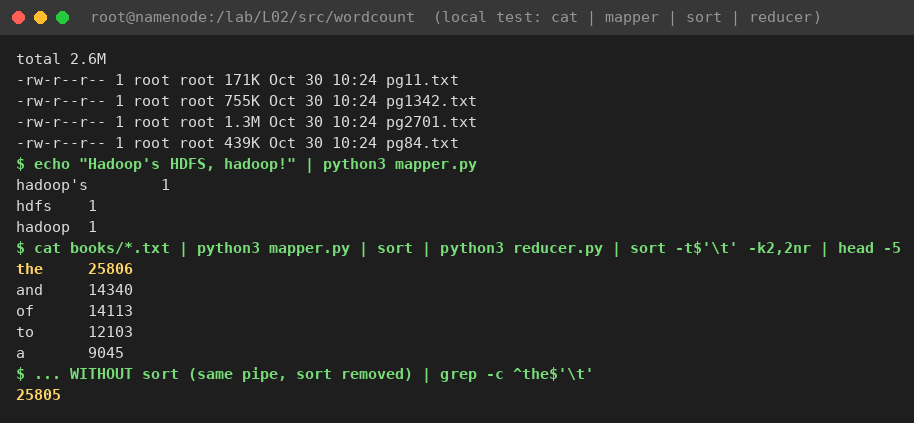
\includegraphics[width=0.85\linewidth,height=\textheight,keepaspectratio]{img/01_wordcount_local_pipe.png}
\caption{Kiểm thử cục bộ đường ống
\texttt{cat\ \textbar{}\ mapper\ \textbar{}\ sort\ \textbar{}\ reducer}\allowbreak{}
trên bốn cuốn sách: top 5 từ và số dòng \texttt{the} khi bỏ
\texttt{sort}.}\label{fig:l02-local-pipe}
\end{figure}

\subsection{Đếm từ trên YARN}\label{sec:l02-wc-yarn}

Sách được đưa lên
\texttt{/}\allowbreak{}\texttt{user/}\allowbreak{}\texttt{root/}\allowbreak{}\texttt{books}\allowbreak{}
và job chạy bằng \texttt{hadoop\ jar\ \$STREAM}\allowbreak{} với
\texttt{-files\ mapper.}\allowbreak{}\texttt{py,}\allowbreak{}\texttt{reducer.}\allowbreak{}\texttt{py}\allowbreak{}
để gửi script tới thư mục làm việc của từng task. Job \texttt{wordcount}
(\texttt{job\_}\allowbreak{}\texttt{1793355278127\_}\allowbreak{}\texttt{0001}\allowbreak{})
chạy thành công với
\texttt{number\ of\ splits:}\allowbreak{}\texttt{4}\allowbreak{}: mỗi
cuốn sách nhỏ hơn một block nên được một split, vì vậy có 4 map task và
1 reduce task theo mặc định (Bảng~\ref{tbl:l02-wc},
Hình~\ref{fig:l02-wc-yarn}). Số khóa vào reducer bằng số dòng đầu ra, và
top 5 đọc từ HDFS giống bản chạy cục bộ.

\begin{longtable}[]{@{}ll@{}}
\caption{\label{tbl:l02-wc}Counter của job đếm từ trên
YARN.}\tabularnewline
\toprule\noalign{}
Counter & Giá trị \\
\midrule\noalign{}
\endfirsthead
\toprule\noalign{}
Counter & Giá trị \\
\midrule\noalign{}
\endhead
\bottomrule\noalign{}
\endlastfoot
Launched map tasks / reduce tasks & 4 / 1 \\
Map input records & 48,749 \\
Map output records & 462,618 \\
Map output bytes & 3,408,811 \\
Map output materialized bytes = Reduce shuffle bytes & 4,334,071 \\
Reduce input groups = Reduce output records & 20,967 \\
HDFS bytes written (\texttt{part-00000}) & 226,341 \\
CPU time spent & 7,010 ms \\
Thời gian lệnh (\texttt{real}) & 23.572 s \\
\end{longtable}

\begin{figure}
\centering
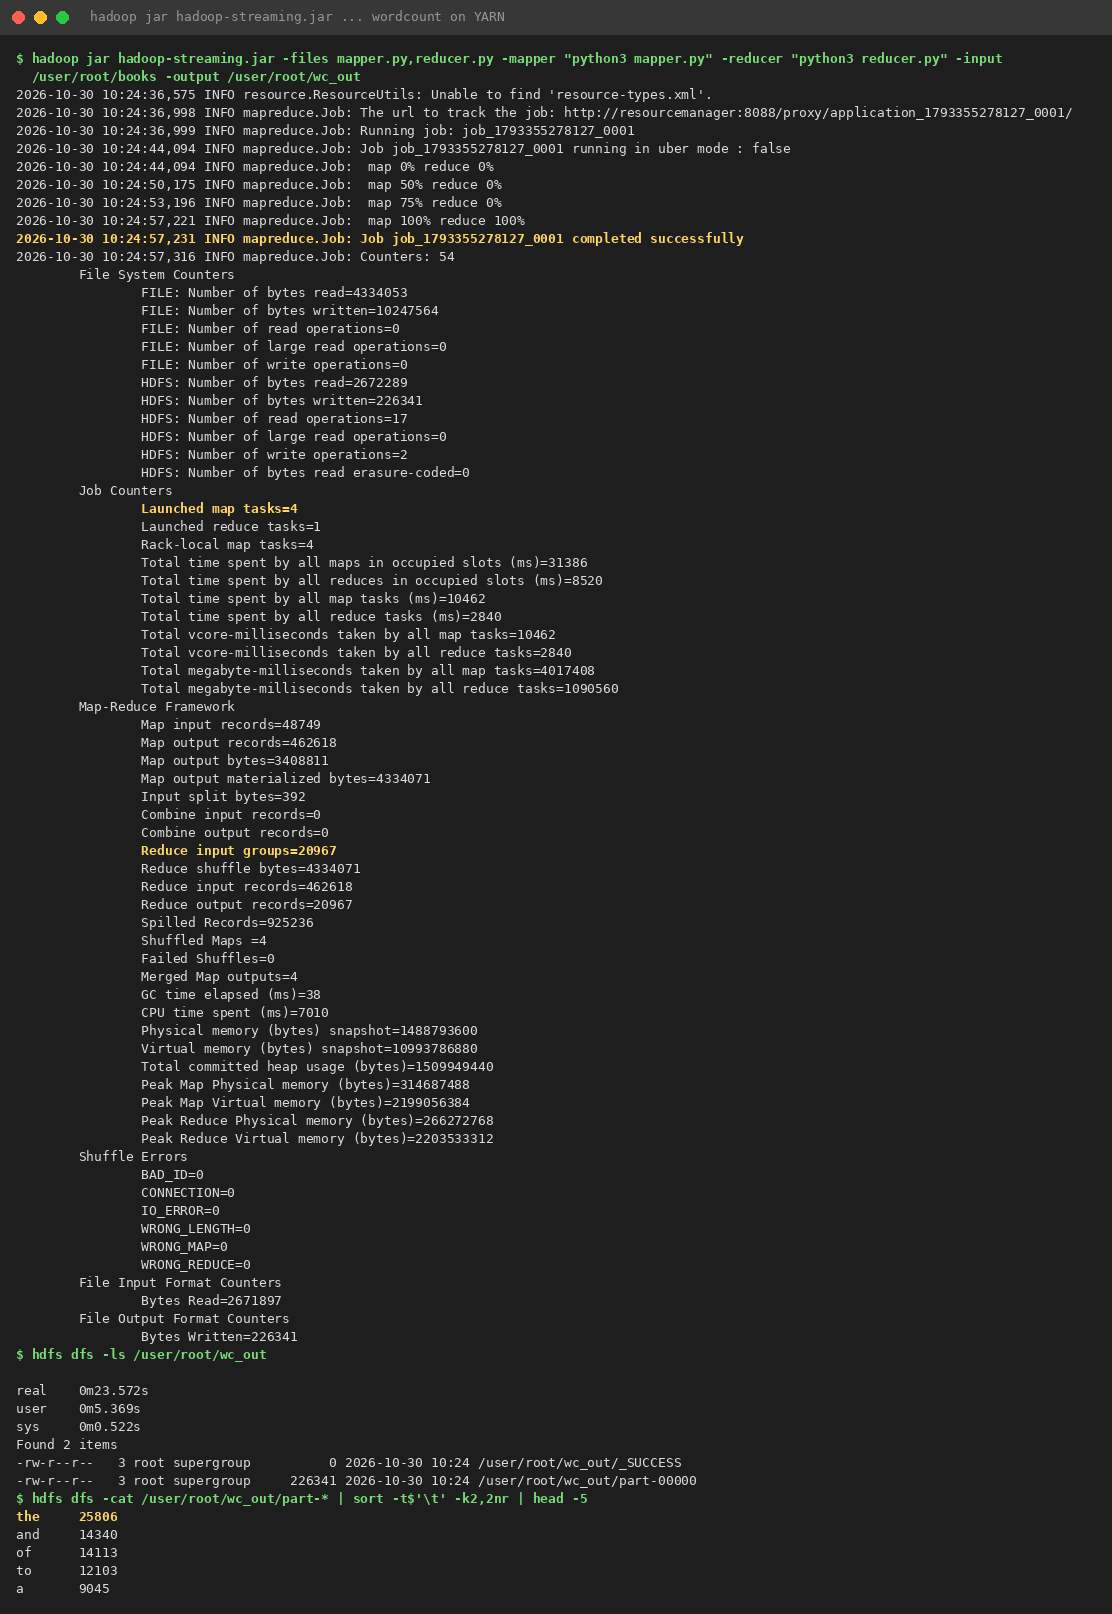
\includegraphics[width=0.85\linewidth,height=\textheight,keepaspectratio]{img/02_wordcount_yarn_counters.png}
\caption{Counter cuối job \texttt{wordcount} trên YARN: 4 map task,
\texttt{Reduce\ input\ groups=}\allowbreak{}\texttt{20967}\allowbreak{}
và top 5 từ đọc từ HDFS.}\label{fig:l02-wc-yarn}
\end{figure}

\subsection{Chuẩn bị dữ liệu taxi và map-side join}\label{sec:l02-zones}

Tệp CSV được đưa lên bằng
\texttt{hdfs\ dfs\ -D\ dfs.}\allowbreak{}\texttt{blocksize=}\allowbreak{}\texttt{16m\ -put}\allowbreak{}
để job có nhiều split hơn. Số block dự kiến là
\(\lceil 92{,}847{,}108 / 16{,}777{,}216 \rceil = \lceil 5.53 \rceil = 6\),
và \texttt{hdfs\ fsck} báo đúng
\texttt{92847108\ bytes,}\allowbreak{}\texttt{\ replicated:}\allowbreak{}\texttt{\ replication=}\allowbreak{}\texttt{3,}\allowbreak{}\texttt{\ 6\ block(s):}\allowbreak{}\texttt{\ OK}\allowbreak{}.

Mapper khu vực nạp
\texttt{taxi\_}\allowbreak{}\texttt{zone\_}\allowbreak{}\texttt{lookup.}\allowbreak{}\texttt{csv}\allowbreak{}
vào một \texttt{dict} rồi đổi \texttt{PULocationID} thành
\texttt{Borough/Zone} ngay khi đọc từng chuyến, nên bảng lớn không phải
shuffle theo khóa nối. Dòng hỏng không làm mapper dừng mà được đếm bằng
cách ghi
\texttt{reporter:}\allowbreak{}\texttt{counter:}\allowbreak{}\texttt{TaxiLab,}\allowbreak{}\texttt{BAD\_}\allowbreak{}\texttt{RECORDS,}\allowbreak{}\texttt{1}\allowbreak{}
ra stderr. Lúc thử cục bộ, mapper chưa đọc được bảng tra cứu vì
\texttt{-files} chỉ có tác dụng trên cluster, nên chúng tôi chép
\texttt{taxi\_}\allowbreak{}\texttt{zone\_}\allowbreak{}\texttt{lookup.}\allowbreak{}\texttt{csv}\allowbreak{}
vào thư mục hiện hành để giả lập distributed cache. Trên 1,000 dòng đầu,
ba khu vực nhiều chuyến nhất là
\texttt{Manhattan/}\allowbreak{}\texttt{East\ Village\ 59}\allowbreak{},
\texttt{Manhattan/}\allowbreak{}\texttt{Lincoln\ Square\ East\ 55}\allowbreak{}
và
\texttt{Manhattan/}\allowbreak{}\texttt{Upper\ West\ Side\ South\ 45}\allowbreak{}.
Khi đưa vào hai dòng hỏng (một dòng \texttt{garbage}, một dòng có
\texttt{PULocationID} không phải số), mapper ghi đúng hai dòng counter
ra stderr (Hình~\ref{fig:l02-taxi-local}). Dữ liệu thật không có dòng
hỏng nào, nên nhóm \texttt{TaxiLab} không xuất hiện trong các job trên
cluster và \texttt{Map\ input\ records}\allowbreak{} bằng
\texttt{Map\ output\ records}\allowbreak{}.

\begin{figure}
\centering
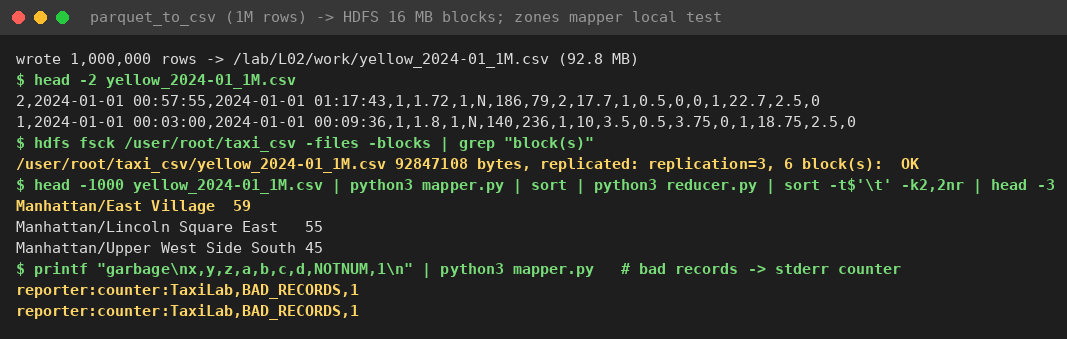
\includegraphics[width=0.85\linewidth,height=\textheight,keepaspectratio]{img/03_taxi_csv_and_zones_local.png}
\caption{Chuyển Parquet sang CSV, 6 block trên HDFS, kiểm thử cục bộ
map-side join trên 1,000 dòng và counter
\texttt{BAD\_RECORDS}.}\label{fig:l02-taxi-local}
\end{figure}

\subsection{Có và không có combiner}\label{sec:l02-combiner}

Combiner là một reducer thu nhỏ chạy trên đầu ra từng map task trước
shuffle. Hadoop có thể gọi nó 0, 1 hay nhiều lần, nên hàm gộp phải có
tính kết hợp, giao hoán và giữ nguyên định dạng {[}1{]}, {[}3{]}. Phép
cộng thỏa điều kiện này nên reducer đếm được dùng lại làm combiner. Hai
job chạy liền nhau, cùng đầu vào, cùng
\texttt{-D\ mapreduce.}\allowbreak{}\texttt{job.}\allowbreak{}\texttt{reduces=}\allowbreak{}\texttt{2}\allowbreak{},
chỉ khác dòng \texttt{-combiner}:

\begin{Shaded}
\begin{Highlighting}[]
\ExtensionTok{hadoop}\NormalTok{ jar }\VariableTok{$STREAM} \AttributeTok{{-}D}\NormalTok{ mapreduce.job.name=zones\_combiner }\AttributeTok{{-}D}\NormalTok{ mapreduce.job.reduces=2 }\DataTypeTok{\textbackslash{}}
  \AttributeTok{{-}files}\NormalTok{ mapper.py,reducer.py,/datasets/data/taxi/taxi\_zone\_lookup.csv }\DataTypeTok{\textbackslash{}}
  \AttributeTok{{-}mapper} \StringTok{"python3 mapper.py"} \AttributeTok{{-}combiner} \StringTok{"python3 reducer.py"} \AttributeTok{{-}reducer} \StringTok{"python3 reducer.py"} \DataTypeTok{\textbackslash{}}
  \AttributeTok{{-}input}\NormalTok{ /user/root/taxi\_csv }\AttributeTok{{-}output}\NormalTok{ /user/root/zones\_out\_combiner}
\end{Highlighting}
\end{Shaded}

Bảng~\ref{tbl:l02-combiner} gồm các counter đề bài yêu cầu cho
\texttt{zones\_}\allowbreak{}\texttt{nocombiner}\allowbreak{}
(\texttt{job\_}\allowbreak{}\texttt{1793355278127\_}\allowbreak{}\texttt{0002}\allowbreak{})
và \texttt{zones\_combiner}
(\texttt{job\_}\allowbreak{}\texttt{1793355278127\_}\allowbreak{}\texttt{0003}\allowbreak{});
Bảng~\ref{tbl:l02-combiner-extra} gồm thêm vài counter lấy từ log đầy
đủ. Wall-clock được tính bằng hiệu thời điểm giữa dòng log
\texttt{Running\ job} và dòng
\texttt{completed\ successfully}\allowbreak{}, không dùng lệnh
\texttt{time}, nên không gồm phần khởi động client.

\begin{longtable}[]{@{}lll@{}}
\caption{\label{tbl:l02-combiner}So sánh counter giữa hai lần chạy không
và có combiner.}\tabularnewline
\toprule\noalign{}
Counter & Không combiner & Có combiner \\
\midrule\noalign{}
\endfirsthead
\toprule\noalign{}
Counter & Không combiner & Có combiner \\
\midrule\noalign{}
\endhead
\bottomrule\noalign{}
\endlastfoot
Launched map tasks & 6 & 6 \\
Map output records & 1,000,000 & 1,000,000 \\
Combine input records & 0 & 1,000,000 \\
Combine output records & 0 & 1,382 \\
Map output materialized bytes & 31,039,071 & 41,169 \\
Reduce shuffle bytes & 31,039,071 & 41,169 \\
Reduce input records & 1,000,000 & 1,382 \\
Wall-clock time & 30.3 s & 33.3 s \\
\end{longtable}

\begin{longtable}[]{@{}lll@{}}
\caption{\label{tbl:l02-combiner-extra}Counter bổ sung của hai lần chạy
khu vực (trích từ \texttt{nocombiner.log} và
\texttt{combiner.log}).}\tabularnewline
\toprule\noalign{}
Counter & Không combiner & Có combiner \\
\midrule\noalign{}
\endfirsthead
\toprule\noalign{}
Counter & Không combiner & Có combiner \\
\midrule\noalign{}
\endhead
\bottomrule\noalign{}
\endlastfoot
Map output bytes & 29,038,999 & 29,038,999 \\
Reduce input groups = Reduce output records & 247 & 247 \\
Spilled Records & 2,000,000 & 2,764 \\
FILE: Number of bytes written & 64,607,796 & 2,614,896 \\
FILE: Number of bytes read & 31,039,011 & 41,109 \\
Total time spent by all map tasks & 17,287 ms & 17,398 ms \\
Total time spent by all reduce tasks & 13,013 ms & 11,353 ms \\
CPU time spent & 15,050 ms & 14,020 ms \\
Shuffled Maps / Merged Map outputs & 12 / 12 & 12 / 12 \\
Killed reduce tasks & 1 & không xuất hiện \\
\end{longtable}

\begin{figure}
\centering
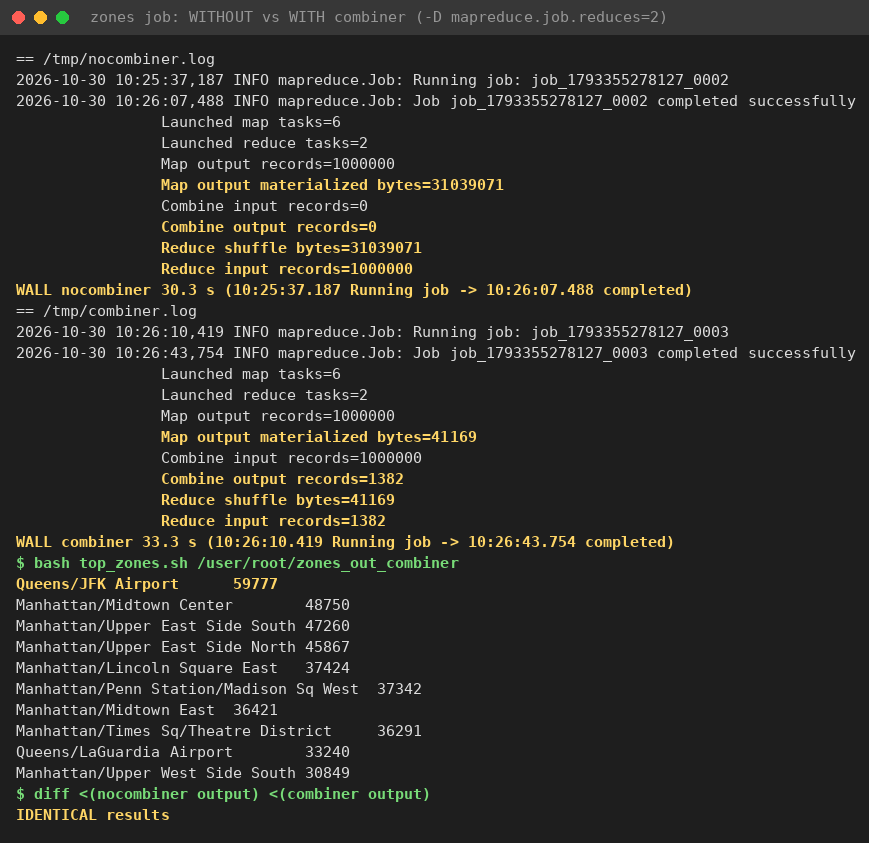
\includegraphics[width=0.85\linewidth,height=\textheight,keepaspectratio]{img/04_combiner_vs_nocombiner_counters.png}
\caption{Trích các counter so sánh từ hai log và top 10 khu vực đón
khách; \texttt{diff} giữa hai đầu ra cho kết quả
IDENTICAL.}\label{fig:l02-combiner-cli}
\end{figure}

\texttt{Map\ output\ bytes}\allowbreak{} không đổi, tức mapper sinh cùng
lượng dữ liệu ở cả hai lần; combiner thu gọn nó trước khi ghi đĩa và
shuffle. Lượng shuffle giảm \(31{,}039{,}071 / 41{,}169 \approx\)
\textbf{754 lần} (khoảng 99.9 \%), số bản ghi tràn đĩa và số byte ghi
đĩa cục bộ giảm cùng cỡ. Cả hai lần đều có 247 khu vực vào reducer và
\texttt{diff} hai đầu ra rỗng (Hình~\ref{fig:l02-combiner-cli}). Ba khu
vực đứng đầu là
\texttt{Queens/}\allowbreak{}\texttt{JFK\ Airport\ 59777}\allowbreak{},
\texttt{Manhattan/}\allowbreak{}\texttt{Midtown\ Center\ 48750}\allowbreak{}
và
\texttt{Manhattan/}\allowbreak{}\texttt{Upper\ East\ Side\ South\ 47260}\allowbreak{}.

Riêng thời gian thì ngược với dự đoán: bản có combiner chậm hơn 3.0 s.
Tổng thời gian map gần như không đổi, chỉ thời gian reduce giảm. Lần
chạy không combiner có
\texttt{Killed\ reduce\ tasks=}\allowbreak{}\texttt{1}\allowbreak{}; đây
là một attempt reduce bị hủy, cả hai reduce task vẫn chạy xong nên kết
quả không bị ảnh hưởng.

\subsection{Giao diện YARN, JobHistory và CLI}\label{sec:l02-ui}

ResourceManager UI liệt kê 3 ứng dụng đã xong (\texttt{wordcount},
\texttt{zones\_}\allowbreak{}\texttt{nocombiner}\allowbreak{},
\texttt{zones\_combiner}), 1 Active Node, Capacity Scheduler và giới hạn
container như ở Bảng~\ref{tbl:l02-env} (Hình~\ref{fig:l02-ui-yarn}).
Danh sách job trên JobHistory ở Hình~\ref{fig:l02-ui-history}.

\begin{figure}
\centering
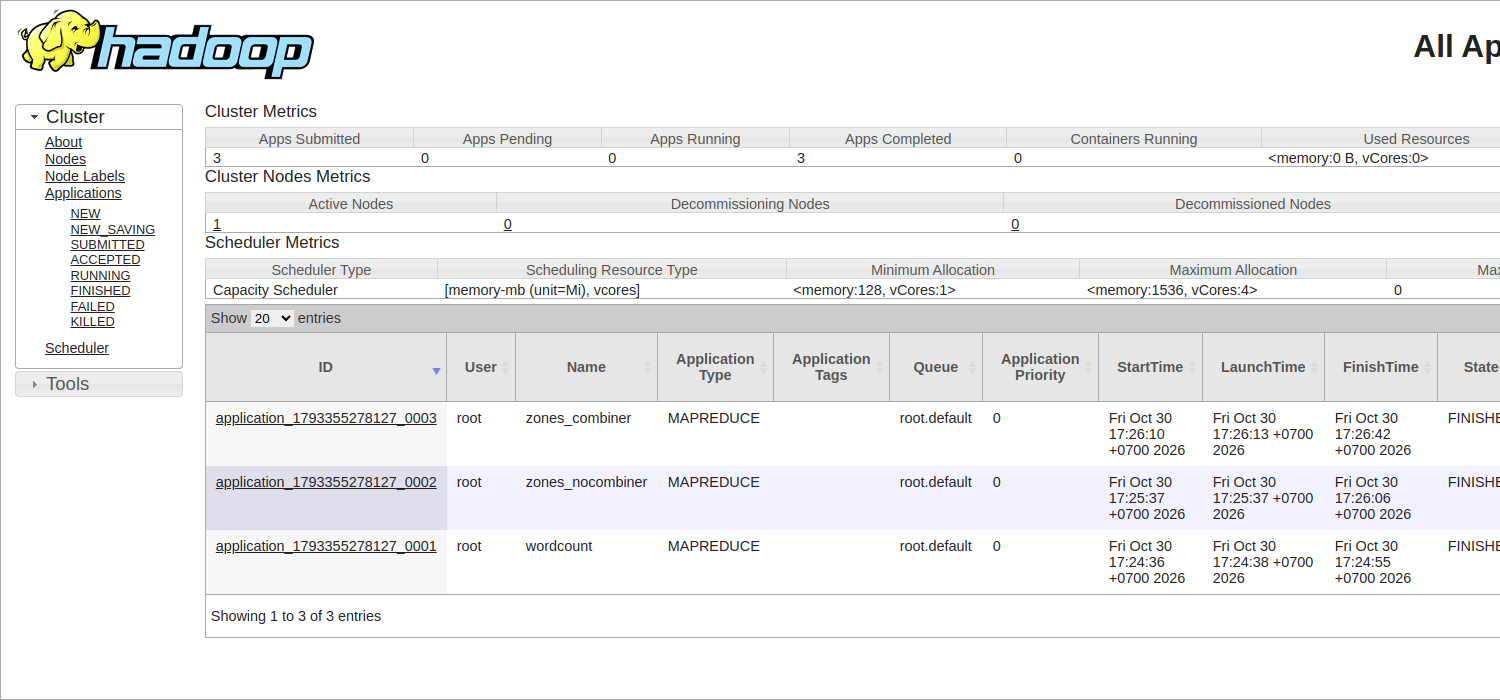
\includegraphics[width=1\linewidth,height=\textheight,keepaspectratio]{img/10_ui_yarn_applications.png}
\caption{YARN ResourceManager UI (cổng 8088): ba ứng dụng MapReduce đã
hoàn thành và các chỉ số cluster.}\label{fig:l02-ui-yarn}
\end{figure}

\begin{figure}
\centering
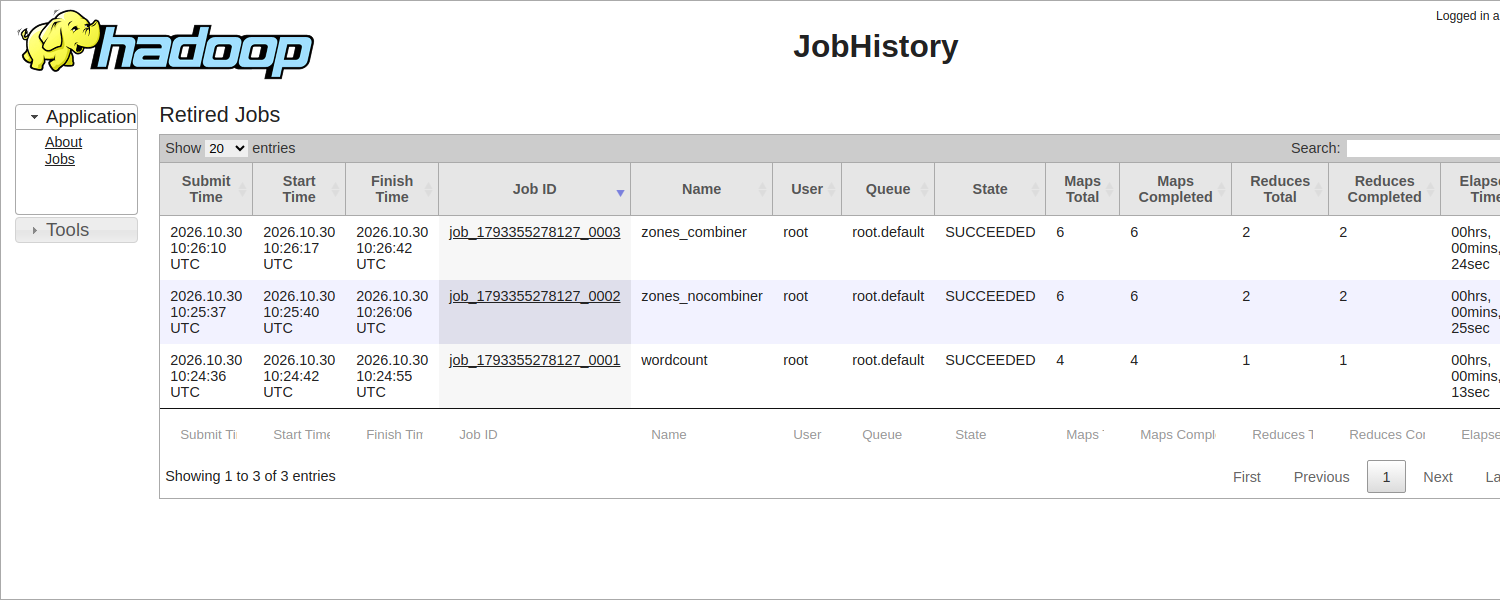
\includegraphics[width=1\linewidth,height=\textheight,keepaspectratio]{img/11_ui_jobhistory_jobs.png}
\caption{JobHistory UI (cổng 19888): danh sách các job đã hoàn
thành.}\label{fig:l02-ui-history}
\end{figure}

Trang tổng quan của
\texttt{job\_}\allowbreak{}\texttt{1793355278127\_}\allowbreak{}\texttt{0003}\allowbreak{}
(Hình~\ref{fig:l02-ui-overview}) ghi SUCCEEDED, không chạy chế độ uber,
Elapsed 24 s, map trung bình 2 s, shuffle trung bình 5 s; cả 6 map và 2
reduce đều thành công, không attempt nào lỗi hay bị hủy. Elapsed ngắn
hơn wall-clock ở Bảng~\ref{tbl:l02-combiner} vì wall-clock còn gồm thời
gian chờ ApplicationMaster khởi động.

\begin{figure}
\centering
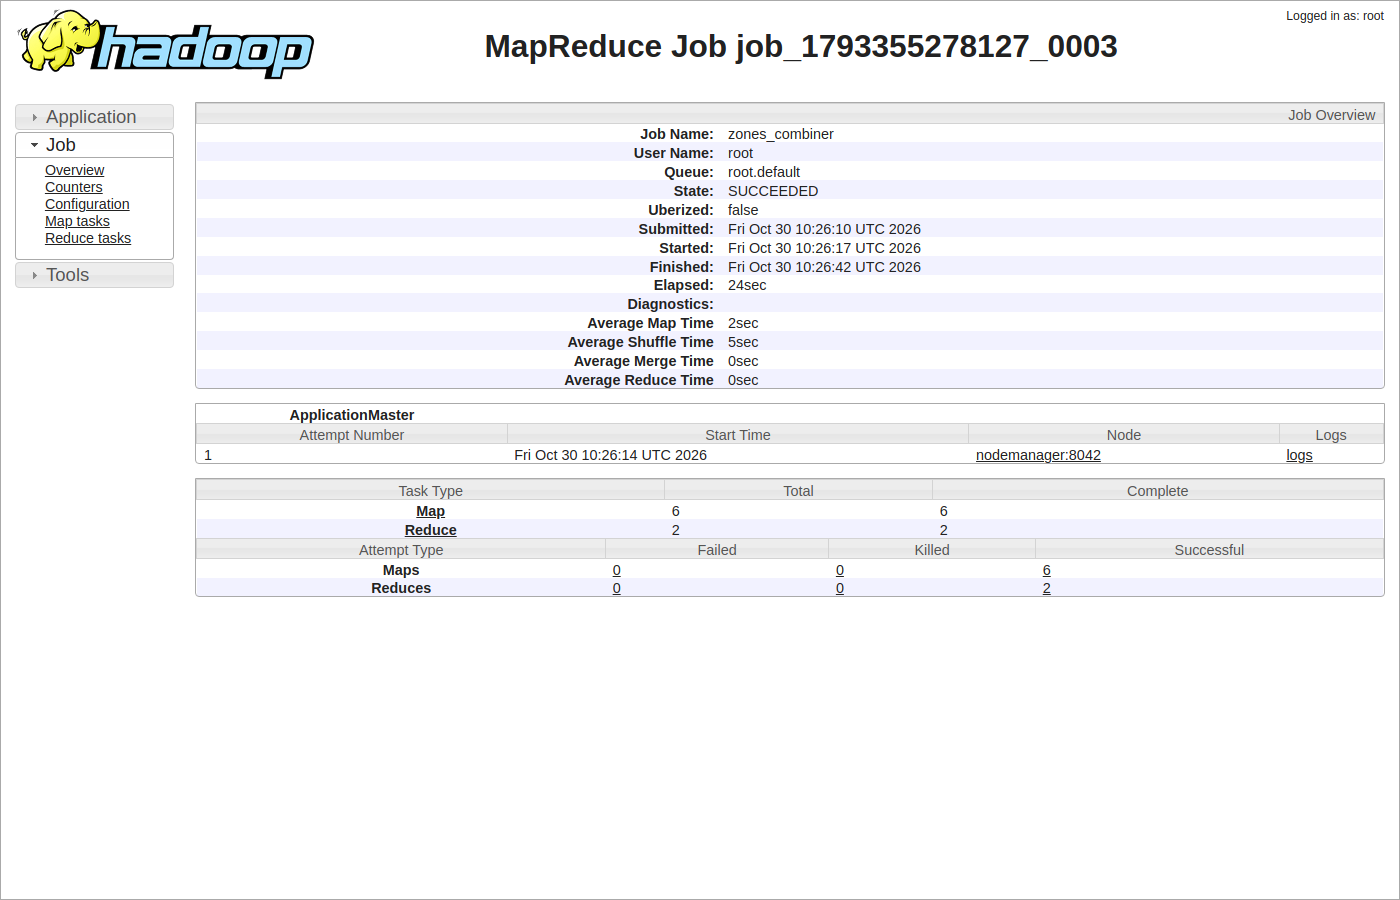
\includegraphics[width=1\linewidth,height=\textheight,keepaspectratio]{img/14_ui_job_combiner_overview.png}
\caption{JobHistory UI: tổng quan job \texttt{zones\_combiner} với 6 map
task, 2 reduce task và thời gian từng pha.}\label{fig:l02-ui-overview}
\end{figure}

Trang Counters của hai job (Hình~\ref{fig:l02-ui-counters-nc},
Hình~\ref{fig:l02-ui-counters-c}) cho đúng các giá trị in trên console.

\begin{figure}
\centering
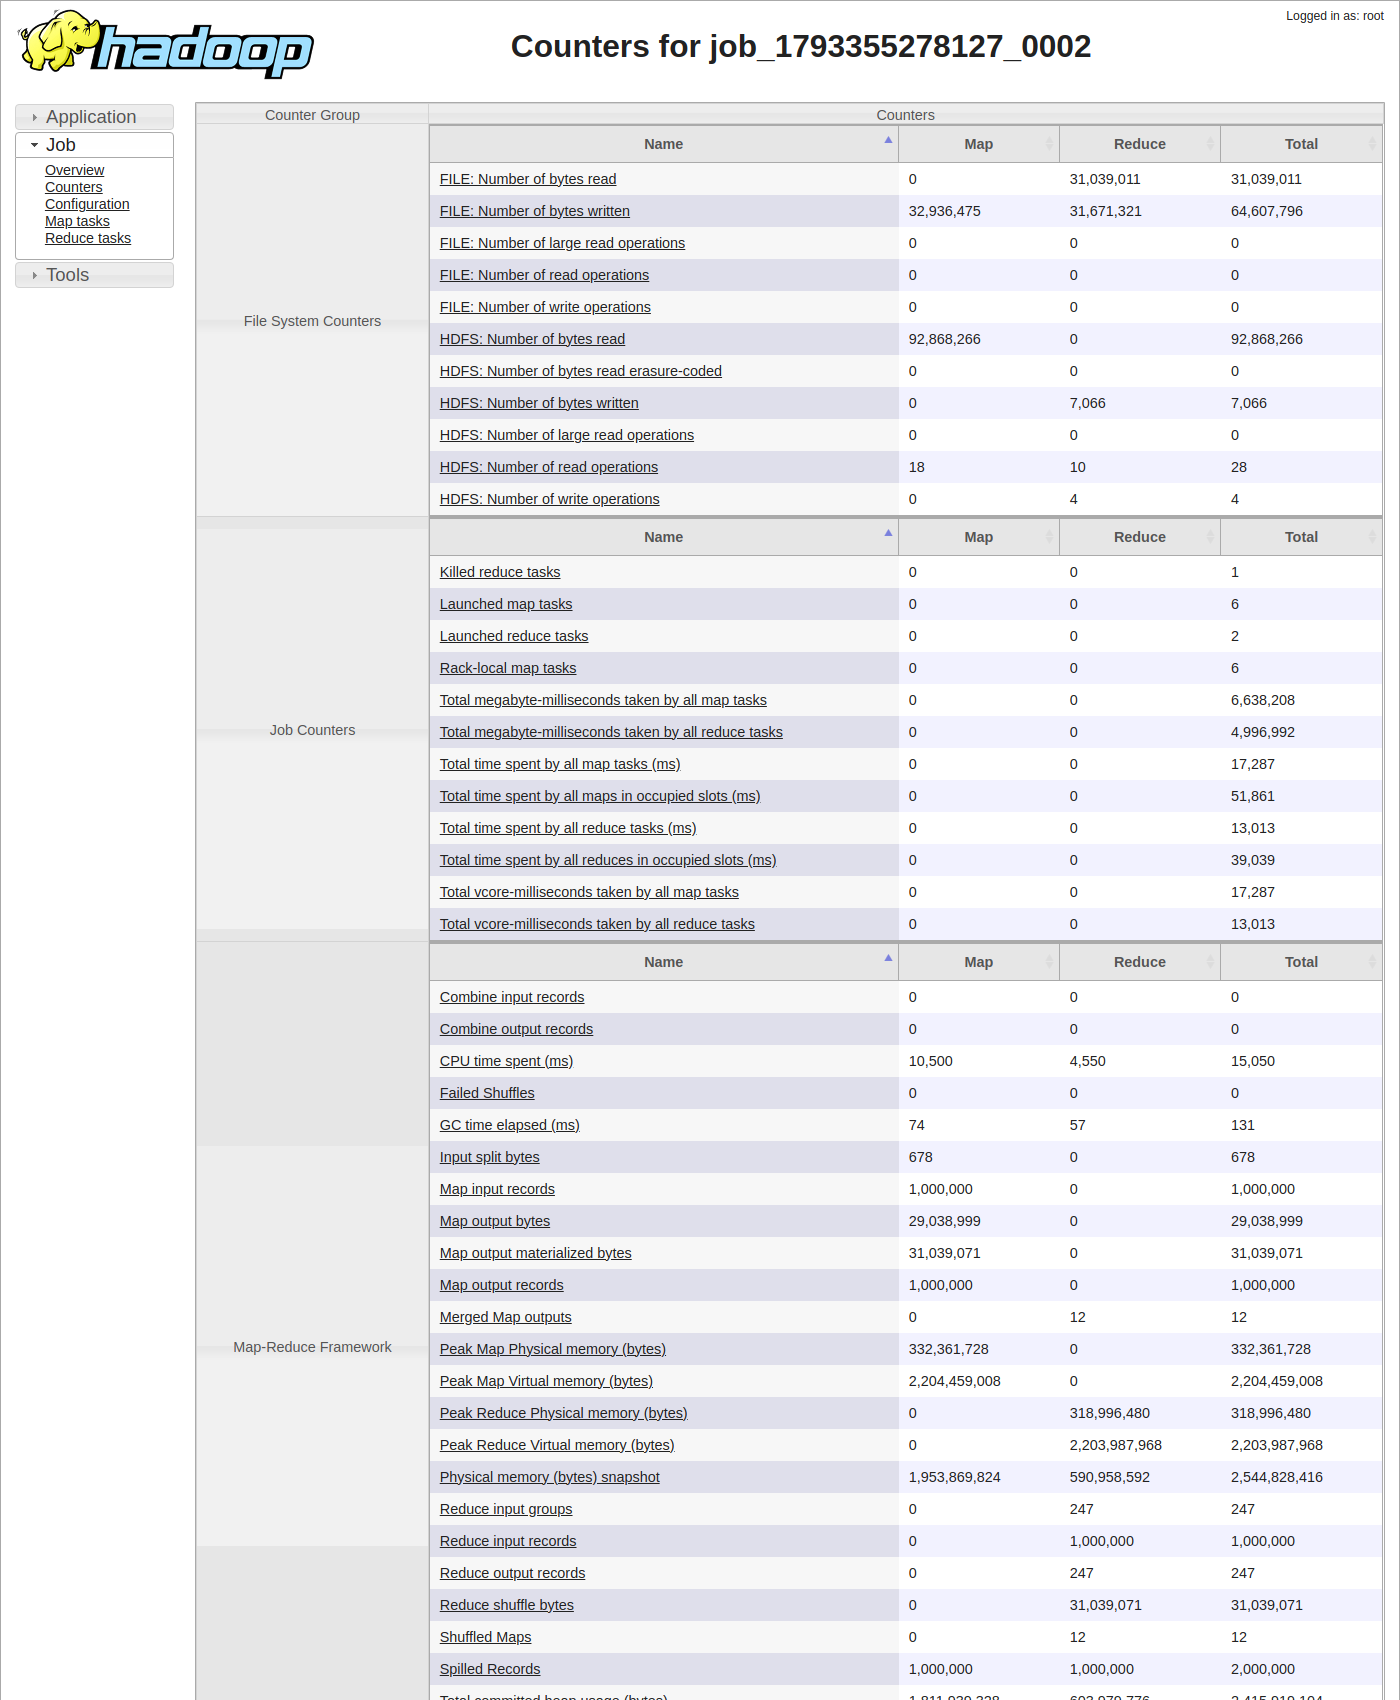
\includegraphics[width=1\linewidth,height=\textheight,keepaspectratio]{img/12_ui_counters_nocombiner.png}
\caption{JobHistory UI: trang Counters của job không
combiner.}\label{fig:l02-ui-counters-nc}
\end{figure}

\begin{figure}
\centering
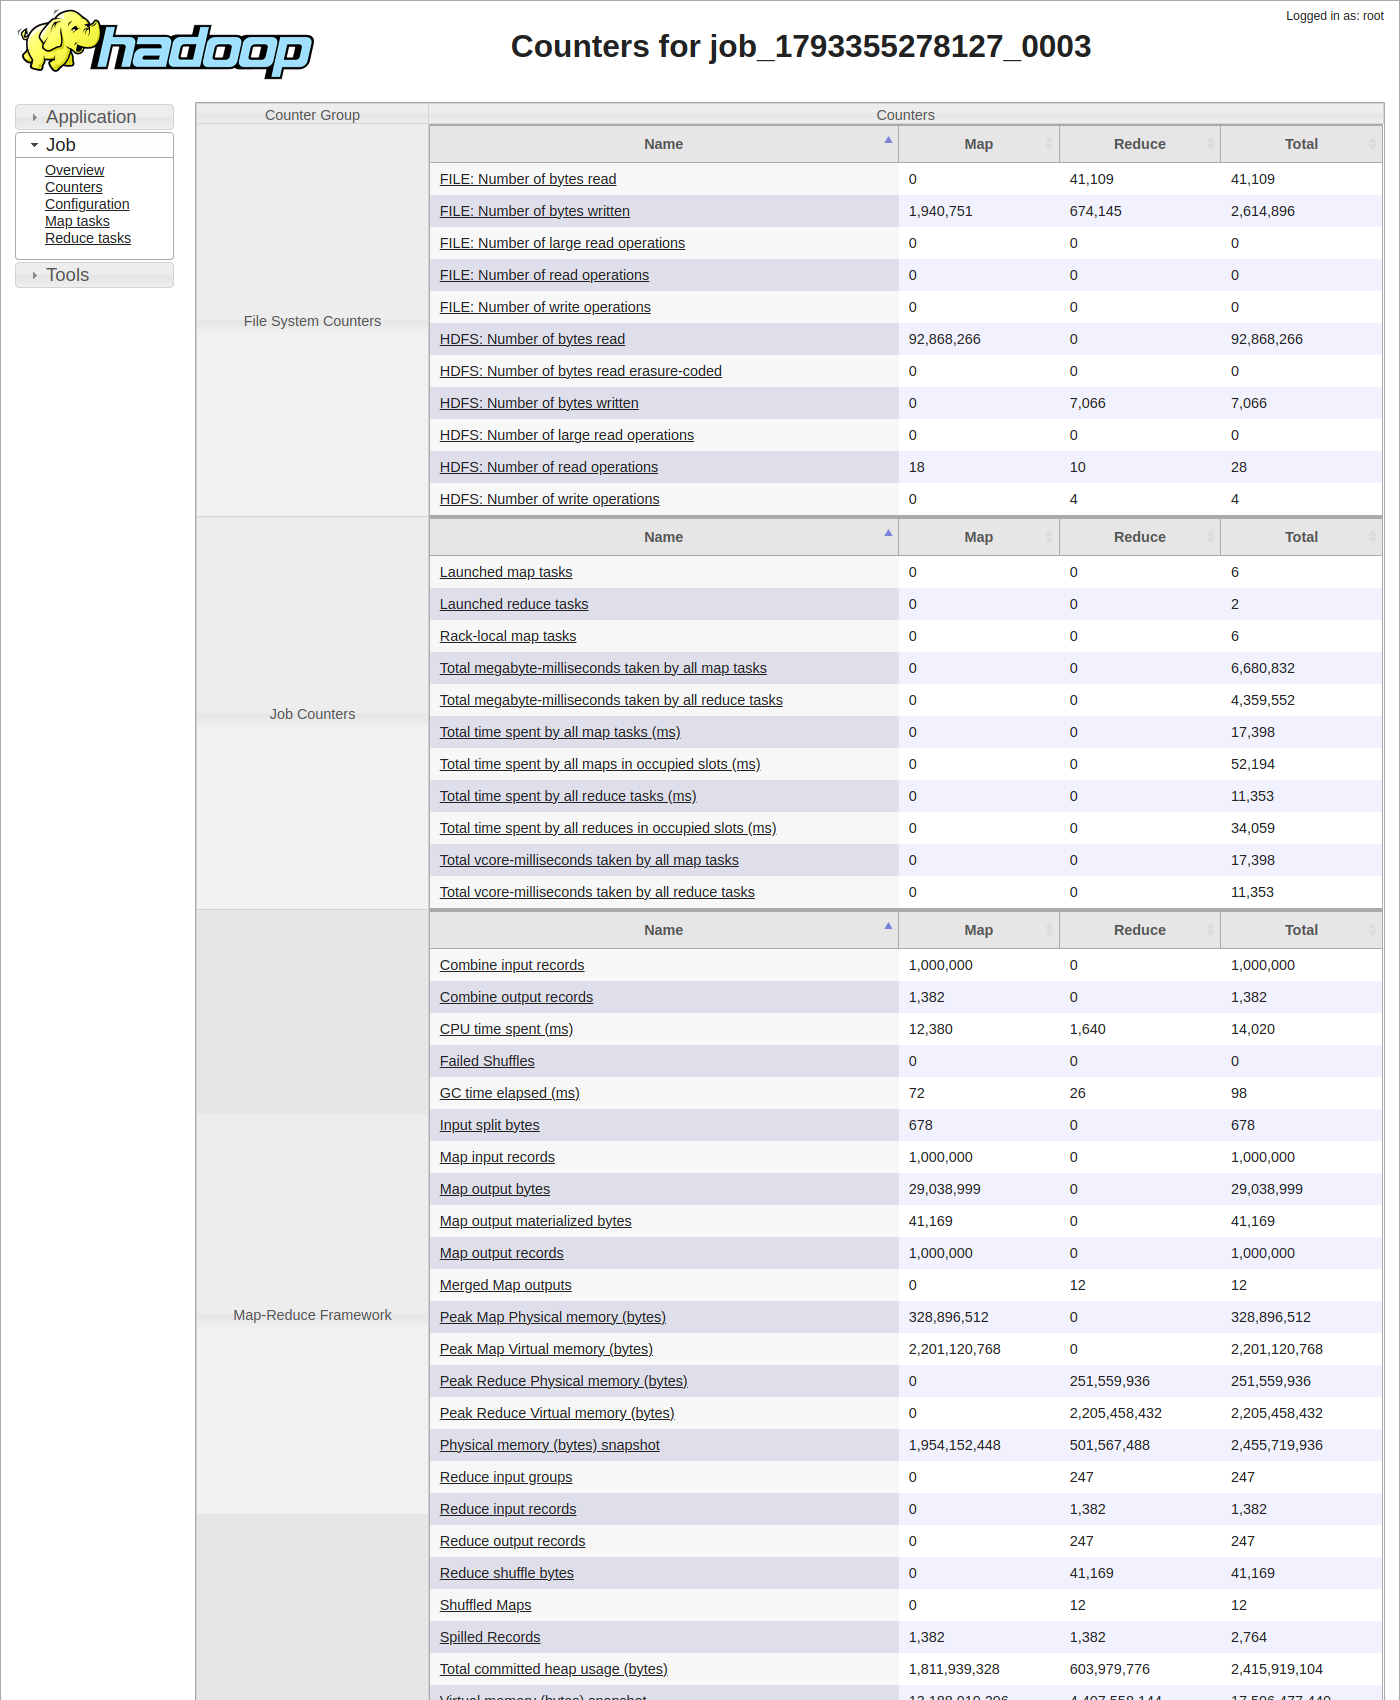
\includegraphics[width=1\linewidth,height=\textheight,keepaspectratio]{img/13_ui_counters_combiner.png}
\caption{JobHistory UI: trang Counters của job có
combiner.}\label{fig:l02-ui-counters-c}
\end{figure}

Trên dòng lệnh,
\texttt{yarn\ application\ -list\ -appStates\ FINISHED}\allowbreak{} cho
3 ứng dụng có Final-State SUCCEEDED, với Tracking-URL trỏ tới
\texttt{historyserver:}\allowbreak{}\texttt{19888}\allowbreak{}, và
\texttt{mapred\ job\ -list\ all}\allowbreak{} báo \texttt{Total\ jobs:3}
(Hình~\ref{fig:l02-yarn-cli}).

\begin{figure}
\centering
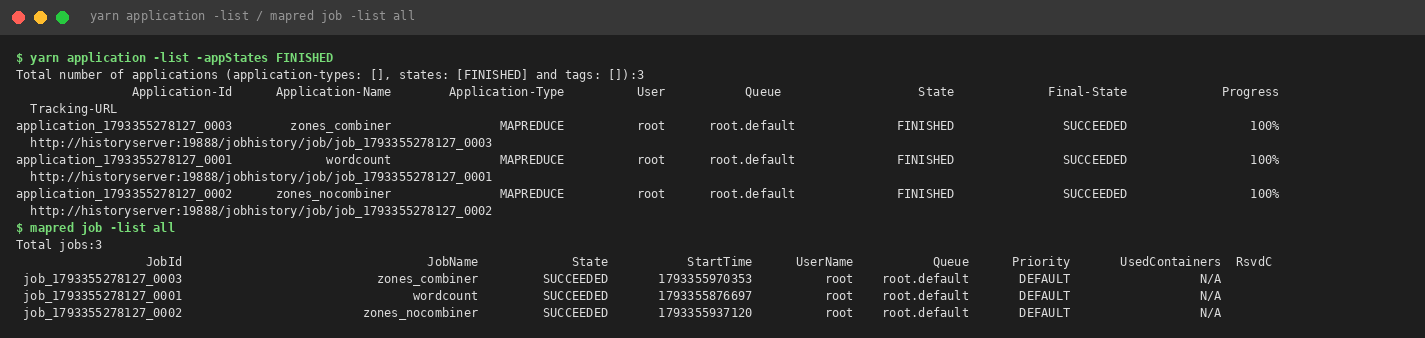
\includegraphics[width=0.85\linewidth,height=\textheight,keepaspectratio]{img/05_yarn_cli.png}
\caption{Kiểm tra các job đã hoàn thành bằng
\texttt{yarn\ application\ -list}\allowbreak{} và
\texttt{mapred\ job\ -list\ all}\allowbreak{}.}\label{fig:l02-yarn-cli}
\end{figure}

\subsection{Mở rộng: giá cước trung bình theo khu
vực}\label{sec:l02-avgfare}

Mapper phát
\texttt{zone\textbackslash{}t\textless{}fare\textgreater{},1}, trong đó
\texttt{fare\_amount} là cột thứ 10. Combiner cộng dồn cặp
\texttt{(sum,\ count)} và xuất đúng định dạng nó nhận vào; reducer cộng
tiếp và chỉ chia \texttt{sum/count} ở bước cuối. Job
\texttt{job\_}\allowbreak{}\texttt{1793355278127\_}\allowbreak{}\texttt{0004}\allowbreak{}
chạy xong với
\texttt{Combine\ input\ records=}\allowbreak{}\texttt{1000000}\allowbreak{},
\texttt{Combine\ output\ records=}\allowbreak{}\texttt{1382}\allowbreak{}
và
\texttt{Reduce\ shuffle\ bytes=}\allowbreak{}\texttt{56289}\allowbreak{}
(Bảng~\ref{tbl:l02-avgfare}, Hình~\ref{fig:l02-avgfare}).

\begin{longtable}[]{@{}lll@{}}
\caption{\label{tbl:l02-avgfare}Giá cước trung bình
(\texttt{fare\_amount}) của 10 khu vực đón khách nhiều chuyến
nhất.}\tabularnewline
\toprule\noalign{}
Khu vực & Giá cước trung bình & Số chuyến \\
\midrule\noalign{}
\endfirsthead
\toprule\noalign{}
Khu vực & Giá cước trung bình & Số chuyến \\
\midrule\noalign{}
\endhead
\bottomrule\noalign{}
\endlastfoot
Queens/JFK Airport & 59.71 & 59,777 \\
Manhattan/Midtown Center & 15.33 & 48,750 \\
Manhattan/Upper East Side South & 11.91 & 47,260 \\
Manhattan/Upper East Side North & 12.49 & 45,867 \\
Manhattan/Lincoln Square East & 13.30 & 37,424 \\
Manhattan/Penn Station/Madison Sq West & 15.72 & 37,342 \\
Manhattan/Midtown East & 14.71 & 36,421 \\
Manhattan/Times Sq/Theatre District & 18.20 & 36,291 \\
Queens/LaGuardia Airport & 40.87 & 33,240 \\
Manhattan/Upper West Side South & 13.36 & 30,849 \\
\end{longtable}

\begin{figure}
\centering
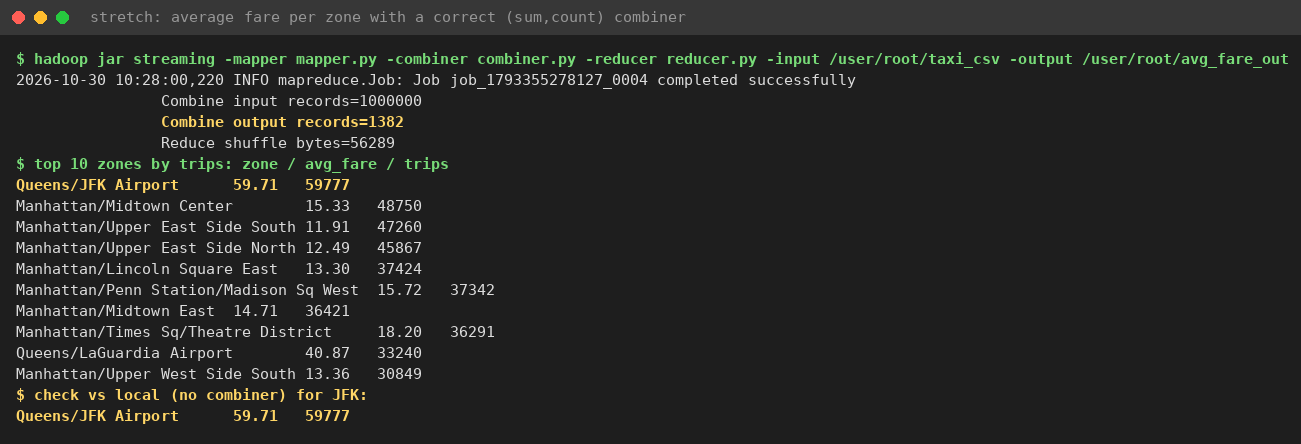
\includegraphics[width=0.85\linewidth,height=\textheight,keepaspectratio]{img/06_stretch_avg_fare.png}
\caption{Job tính giá cước trung bình theo khu vực với combiner
\texttt{(sum,\ count)} và đối chiếu JFK với bản chạy không
combiner.}\label{fig:l02-avgfare}
\end{figure}

Tính lại JFK bằng bản cục bộ không combiner cũng được 59.71 trên 59,777
chuyến, và số chuyến từng khu vực khớp với job đếm ở
Mục~\ref{sec:l02-combiner}. Số bản ghi shuffle vẫn là 1,382 nhưng số
byte nhiều hơn vì mỗi giá trị mang thêm một tổng số thực. Hai sân bay có
giá trung bình cao hơn hẳn các khu vực Manhattan, do chuyến từ sân bay
thường dài hơn.

\section{Trả lời câu hỏi checkpoint}\label{sec:l02-discussion}

\subsection{Trong đường ống cục bộ, lệnh nào làm việc của shuffle, và
thiếu nó thì sao?}\label{sec:l02-q1}

Lệnh \texttt{sort}. Trên cluster, shuffle phân vùng đầu ra map theo khóa
rồi merge-sort ở reducer, nên các bản ghi cùng khóa luôn nằm liền nhau
{[}3{]}; \texttt{sort} cho đúng bảo đảm đó. Không có nó, reducer gặp
cùng một từ ở nhiều đoạn rời nhau và in ra nhiều lần với số đếm cục bộ,
như các dòng \texttt{the} ở Hình~\ref{fig:l02-local-pipe}.

\subsection{\texorpdfstring{Vì sao reducer Streaming phải tự giữ
\texttt{current\_key}?}{Vì sao reducer Streaming phải tự giữ current\_key?}}\label{sec:l02-q2}

Streaming chỉ đưa cho reducer các dòng văn bản đã sắp xếp; nhóm
\texttt{(key,}\allowbreak{}\texttt{\ Iterable\textless{}values\textgreater{})}\allowbreak{}
chỉ có trong API Java {[}2{]}. Reducer Python phải so khóa với
\texttt{current\_key}, in tổng khi khóa đổi và nhớ in khóa cuối sau vòng
lặp (Phụ lục). Quên bước cuối thì mất từ cuối cùng. Reducer của bài
không mắc lỗi này: \texttt{Reduce\ output\ records}\allowbreak{} bằng
\texttt{Reduce\ input\ groups}\allowbreak{} ở Bảng~\ref{tbl:l02-wc}.

\subsection{Job taxi có bao nhiêu map task, bao nhiêu reduce task, và vì
sao?}\label{sec:l02-q3}

Job taxi có 6 map task vì tệp CSV nằm trong 6 block 16 MB và mỗi block
là một split (log ghi
\texttt{number\ of\ splits:}\allowbreak{}\texttt{6}\allowbreak{},
Mục~\ref{sec:l02-zones}); job đếm từ chỉ có 4 vì mỗi cuốn sách nhỏ hơn
một block. Số reduce task là 2 vì chúng tôi đặt
\texttt{-D\ mapreduce.}\allowbreak{}\texttt{job.}\allowbreak{}\texttt{reduces=}\allowbreak{}\texttt{2}\allowbreak{}.
Con số này do người dùng chọn chứ không suy ra từ dữ liệu, job đếm từ để
mặc định là 1. Với 2 reducer, mỗi map task tạo hai phân vùng, nên
\texttt{Shuffled\ Maps} bằng \(6 \times 2 = 12\)
(Bảng~\ref{tbl:l02-combiner-extra}). NodeManager chỉ chạy hai task 384
MB cùng lúc nên 6 map chạy thành nhiều đợt; log thể hiện qua tiến độ map
tăng dần 17 \%, 33 \%, 50 \%, 67 \%, 83 \% rồi 100 \%.

\subsection{\texorpdfstring{Combiner giảm
\texttt{Reduce\ shuffle\ bytes}\allowbreak{} bao nhiêu lần, và vì sao
đầu ra combiner xấp xỉ số khu vực nhân số map
task?}{Combiner giảm Reduce shuffle bytes bao nhiêu lần, và vì sao đầu ra combiner xấp xỉ số khu vực nhân số map task?}}\label{sec:l02-q4}

Khoảng 754 lần (Mục~\ref{sec:l02-combiner}). Combiner chạy riêng trên
đầu ra từng map task, và mỗi task chỉ xuất một bản ghi cho mỗi khu vực
nó gặp. Toàn bộ dữ liệu có 247 khu vực, còn mỗi task ra trung bình
\(1{,}382 / 6 \approx 230\) bản ghi, tức mỗi split gặp gần hết các khu
vực. Chỉ các tổng cục bộ này đi qua shuffle, nên
\texttt{Reduce\ input\ records}\allowbreak{} cũng chỉ còn bằng
\texttt{Combine\ output\ records}\allowbreak{}
(Bảng~\ref{tbl:l02-combiner}).

\subsection{Vì sao combiner không làm job nhanh hơn ở đây, và khi nào nó
có ích rõ?}\label{sec:l02-q5}

Trên một máy, shuffle chỉ là chép dữ liệu qua đĩa cục bộ hoặc loopback,
gần như không tốn gì, trong khi combiner thêm một tiến trình Python phải
đọc, phân tích và sắp xếp lại toàn bộ bản ghi đầu ra map. Tổng thời gian
map không giảm, còn phần tiết kiệm ở reduce, khoảng 1.7 s
(Bảng~\ref{tbl:l02-combiner-extra}), không bù được thời gian khởi động
và dao động khi lập lịch container. Mỗi cấu hình mới chạy một lần nên
chênh lệch 3.0 s chưa đủ để kết luận combiner làm chậm; bản tham chiếu
của đề bài cũng ghi khoảng 28 s và 37 s. Trên cluster thật, shuffle đi
qua mạng và mỗi reducer phải merge hàng GB từ hàng trăm mapper. Khi đó
việc bỏ được gần hết lượng shuffle và số bản ghi tràn đĩa sẽ lớn hơn
nhiều so với chi phí CPU của combiner.

\subsection{Có dùng lại reducer ``trung bình'' làm combiner được
không?}\label{sec:l02-q6}

Không được. Trung bình của các trung bình sai khi các phân vùng có số
bản ghi khác nhau: trung bình của \(\{10\}\) và \(\{20, 30\}\) là
\((10+20+30)/3 = 20\), còn trung bình hai trung bình cục bộ là
\((10 + 25)/2 = 17.5\). Reducer trung bình còn xuất ra một số thực, khác
định dạng đầu vào, nên không gộp tiếp được khi Hadoop gọi combiner nhiều
lần. Cách đúng là để combiner phát \texttt{(sum,\ count)} và chỉ reducer
mới chia. Phần mở rộng làm theo cách này và kết quả JFK khớp với bản
không combiner (Mục~\ref{sec:l02-avgfare}).

\subsection{Map-side join trong bài hoạt động thế nào, và khi nào nó
không còn hợp?}\label{sec:l02-q7}

Bảng
\texttt{taxi\_}\allowbreak{}\texttt{zone\_}\allowbreak{}\texttt{lookup.}\allowbreak{}\texttt{csv}\allowbreak{}
được gửi tới mọi task qua \texttt{-files}, mỗi mapper nạp vào bộ nhớ và
tra cứu ngay khi đọc chuyến (Mục~\ref{sec:l02-zones}), nên phép nối xong
ở pha map. Cách này không còn hợp khi bảng ``nhỏ'' không vừa thoải mái
trong bộ nhớ task (ở đây mỗi task chỉ có 384 MB), hoặc khi gửi bảng tới
mọi task tốn hơn cả shuffle. Khi đó phải dùng reduce-side join, tức
shuffle cả hai tập theo khóa nối {[}3{]}. Spark gọi ý tưởng thứ nhất là
broadcast join, sẽ gặp lại ở L06.

\subsection{\texorpdfstring{Counter \texttt{BAD\_RECORDS} hiện ở đâu, và
vì sao nên đếm dòng hỏng thay vì cho job
dừng?}{Counter BAD\_RECORDS hiện ở đâu, và vì sao nên đếm dòng hỏng thay vì cho job dừng?}}\label{sec:l02-q8}

Counter nằm trong job counters, nhóm \texttt{TaxiLab}: phần in ra
console cuối job và mục Counters trên JobHistory UI. Nó chỉ hiện khi có
ít nhất một dòng hỏng; dữ liệu trong bài không có dòng hỏng nên chỉ thấy
được ở phép thử cục bộ (Hình~\ref{fig:l02-taxi-local}). Một job xử lý
hàng tỷ dòng không nên chết vì vài dòng lỗi và bỏ phí mọi công việc đã
làm. Đếm dòng hỏng vẫn cho thấy vấn đề chất lượng dữ liệu, và có thể đặt
ngưỡng để cảnh báo hoặc dừng job khi số dòng hỏng quá nhiều.

\section{Kết luận}\label{sec:l02-conclusion}

Bài đã hoàn thành các task của đề: mapper và reducer đếm từ cho cùng top
5 khi chạy cục bộ và trên YARN, mapper khu vực có map-side join và
counter dòng hỏng, bảng counter so sánh có và không có combiner, kiểm
tra job trên hai giao diện web và CLI, cùng phần mở rộng giá cước trung
bình với combiner \texttt{(sum,\ count)}. Combiner giảm dữ liệu shuffle
khoảng 754 lần mà không đổi kết quả, nhưng không làm job nhanh hơn;
chúng tôi cho rằng lý do nằm ở môi trường một máy chứ không phải ở
combiner. Hạn chế chính là mọi thứ chạy trên một NodeManager, shuffle
không đi qua mạng thật, mỗi cấu hình chỉ chạy một lần, và
\texttt{BAD\_RECORDS} mới được kiểm chứng ở chế độ cục bộ.

\section*{Tài liệu tham khảo}\label{tuxe0i-liux1ec7u-tham-khux1ea3o}
\addcontentsline{toc}{section}{Tài liệu tham khảo}

{[}1{]} J. Dean and S. Ghemawat, ``MapReduce: Simplified Data Processing
on Large Clusters,'' in \emph{Proc. 6th USENIX Symposium on Operating
Systems Design and Implementation (OSDI)}, 2004.

{[}2{]} Apache Software Foundation, ``Hadoop Streaming,'' Apache Hadoop
documentation.
https://hadoop.apache.org/docs/stable/hadoop-streaming/HadoopStreaming.html

{[}3{]} T. White, \emph{Hadoop: The Definitive Guide}, 4th
ed.~Sebastopol, CA, USA: O'Reilly Media, 2015.

\section*{Phụ lục: Trích đoạn mã
nguồn}\label{phux1ee5-lux1ee5c-truxedch-ux111oux1ea1n-muxe3-nguux1ed3n}
\addcontentsline{toc}{section}{Phụ lục: Trích đoạn mã nguồn}

Mã đầy đủ và log của từng task nằm trong \texttt{submission/L02/}
(Bảng~\ref{tbl:l02-files}).

\begin{longtable}[]{@{}
  >{\raggedright\arraybackslash}p{(\linewidth - 2\tabcolsep) * \real{0.5000}}
  >{\raggedright\arraybackslash}p{(\linewidth - 2\tabcolsep) * \real{0.5000}}@{}}
\caption{\label{tbl:l02-files}Danh mục tệp nộp kèm trong
\texttt{submission/L02/}.}\tabularnewline
\toprule\noalign{}
\begin{minipage}[b]{\linewidth}\raggedright
Tệp
\end{minipage} & \begin{minipage}[b]{\linewidth}\raggedright
Nội dung
\end{minipage} \\
\midrule\noalign{}
\endfirsthead
\toprule\noalign{}
\begin{minipage}[b]{\linewidth}\raggedright
Tệp
\end{minipage} & \begin{minipage}[b]{\linewidth}\raggedright
Nội dung
\end{minipage} \\
\midrule\noalign{}
\endhead
\bottomrule\noalign{}
\endlastfoot
\texttt{wc\_mapper.py}, \texttt{wc\_reducer.py},
\texttt{zones\_mapper.py} & Mapper/reducer đếm từ, mapper khu vực \\
\texttt{stretch\_}\allowbreak{}\texttt{avg\_}\allowbreak{}\texttt{fare/}\allowbreak{}
& Mapper, combiner, reducer giá cước trung bình \\
\texttt{01\_}\allowbreak{}\texttt{local\_}\allowbreak{}\texttt{pipe.}\allowbreak{}\texttt{txt}\allowbreak{}
đến
\texttt{06\_}\allowbreak{}\texttt{stretch\_}\allowbreak{}\texttt{avg\_}\allowbreak{}\texttt{fare.}\allowbreak{}\texttt{txt}\allowbreak{}
& Log từng task \\
\texttt{nocombiner.log}, \texttt{combiner.log} & Log đầy đủ hai job khu
vực \\
\end{longtable}

Reducer đếm từ (\texttt{wc\_reducer.py}) tự nhận ra chỗ đổi khóa và in
thêm khóa cuối cùng sau vòng lặp.

\begin{Shaded}
\begin{Highlighting}[]
\NormalTok{current\_word, current\_count }\OperatorTok{=} \VariableTok{None}\NormalTok{, }\DecValTok{0}
\ControlFlowTok{for}\NormalTok{ line }\KeywordTok{in}\NormalTok{ sys.stdin:}
\NormalTok{    word, \_, count }\OperatorTok{=}\NormalTok{ line.rstrip(}\StringTok{"}\CharTok{\textbackslash{}n}\StringTok{"}\NormalTok{).partition(}\StringTok{"}\CharTok{\textbackslash{}t}\StringTok{"}\NormalTok{)}
\NormalTok{    count }\OperatorTok{=} \BuiltInTok{int}\NormalTok{(count)}
    \ControlFlowTok{if}\NormalTok{ word }\OperatorTok{==}\NormalTok{ current\_word:}
\NormalTok{        current\_count }\OperatorTok{+=}\NormalTok{ count}
    \ControlFlowTok{else}\NormalTok{:}
        \ControlFlowTok{if}\NormalTok{ current\_word }\KeywordTok{is} \KeywordTok{not} \VariableTok{None}\NormalTok{:}
            \BuiltInTok{print}\NormalTok{(}\SpecialStringTok{f"}\SpecialCharTok{\{}\NormalTok{current\_word}\SpecialCharTok{\}}\CharTok{\textbackslash{}t}\SpecialCharTok{\{}\NormalTok{current\_count}\SpecialCharTok{\}}\SpecialStringTok{"}\NormalTok{)}
\NormalTok{        current\_word, current\_count }\OperatorTok{=}\NormalTok{ word, count}
\ControlFlowTok{if}\NormalTok{ current\_word }\KeywordTok{is} \KeywordTok{not} \VariableTok{None}\NormalTok{:  }\CommentTok{\# the last word\textquotesingle{}s total}
    \BuiltInTok{print}\NormalTok{(}\SpecialStringTok{f"}\SpecialCharTok{\{}\NormalTok{current\_word}\SpecialCharTok{\}}\CharTok{\textbackslash{}t}\SpecialCharTok{\{}\NormalTok{current\_count}\SpecialCharTok{\}}\SpecialStringTok{"}\NormalTok{)}
\end{Highlighting}
\end{Shaded}

Mapper khu vực (\texttt{zones\_mapper.py}) nạp bảng tra cứu, báo dòng
hỏng qua stderr và phát \texttt{zone\textbackslash{}t1}.

\begin{Shaded}
\begin{Highlighting}[]
\NormalTok{zones }\OperatorTok{=}\NormalTok{ \{\}}
\ControlFlowTok{if}\NormalTok{ os.path.exists(}\StringTok{"taxi\_zone\_lookup.csv"}\NormalTok{):}
    \ControlFlowTok{with} \BuiltInTok{open}\NormalTok{(}\StringTok{"taxi\_zone\_lookup.csv"}\NormalTok{, newline}\OperatorTok{=}\StringTok{""}\NormalTok{) }\ImportTok{as}\NormalTok{ f:}
        \ControlFlowTok{for}\NormalTok{ row }\KeywordTok{in}\NormalTok{ csv.DictReader(f):}
\NormalTok{            zones[row[}\StringTok{"LocationID"}\NormalTok{]] }\OperatorTok{=} \SpecialStringTok{f"}\SpecialCharTok{\{}\NormalTok{row[}\StringTok{\textquotesingle{}Borough\textquotesingle{}}\NormalTok{]}\SpecialCharTok{\}}\SpecialStringTok{/}\SpecialCharTok{\{}\NormalTok{row[}\StringTok{\textquotesingle{}Zone\textquotesingle{}}\NormalTok{]}\SpecialCharTok{\}}\SpecialStringTok{"}
\ControlFlowTok{for}\NormalTok{ line }\KeywordTok{in}\NormalTok{ sys.stdin:}
\NormalTok{    fields }\OperatorTok{=}\NormalTok{ line.rstrip(}\StringTok{"}\CharTok{\textbackslash{}n}\StringTok{"}\NormalTok{).split(}\StringTok{","}\NormalTok{)}
    \ControlFlowTok{if} \BuiltInTok{len}\NormalTok{(fields) }\OperatorTok{\textless{}=}\NormalTok{ PU\_COL }\KeywordTok{or} \KeywordTok{not}\NormalTok{ fields[PU\_COL].strip().isdigit():}
\NormalTok{        sys.stderr.write(}\StringTok{"reporter:counter:TaxiLab,BAD\_RECORDS,1}\CharTok{\textbackslash{}n}\StringTok{"}\NormalTok{)}
        \ControlFlowTok{continue}
\NormalTok{    pu }\OperatorTok{=}\NormalTok{ fields[PU\_COL].strip()}
    \BuiltInTok{print}\NormalTok{(}\SpecialStringTok{f"}\SpecialCharTok{\{}\NormalTok{zones}\SpecialCharTok{.}\NormalTok{get(pu, pu)}\SpecialCharTok{\}}\CharTok{\textbackslash{}t}\SpecialStringTok{1"}\NormalTok{)}
\end{Highlighting}
\end{Shaded}


\end{document}
